\subsection{SP2: reclutamiento heterogéneo por capacidad efectiva}
\label{sec:resultados-sp2}

\subsubsection{Problema y diferencia respecto de SP1}

SP1 cuenta robots intercambiables. SP2 cambia la unidad de decisión: un robot $i$
posee capacidad nominal $c_i$, pero su contribución a la carga $k$ es
\begin{equation}
 e_{ik}=c_i\eta_{ik},\qquad 0\leq\eta_{ik}\leq1,
 \label{eq:sp2-effective-pair}
\end{equation}
donde $\eta_{ik}$ resume batería, distancia, alineación y disponibilidad durante el
instante de decisión. Dos robots con el mismo $c_i$ pueden aportar cantidades distintas
a cargas diferentes. Para $z_{ik}\in\{0,1\}$ y demanda $D_k$, la capacidad reclutada es
$S_k(z)=\sum_i e_{ik}z_{ik}$ y la carga queda servida si $S_k(z)\geq D_k$.
Cada robot atiende como máximo una carga:
\begin{equation}
 \sum_{k=1}^{K}z_{ik}\leq1,
 \qquad
 y_kD_k\leq\sum_{i=1}^{N}e_{ik}z_{ik},
 \qquad y_k\in\{0,1\}.
 \label{eq:sp2-integer-constraints}
\end{equation}
El objetivo de referencia combina cargas completas, cobertura parcial y desplazamiento:
\begin{equation}
 \max_{z,y,u}\;
 \sum_kw_ky_k+\rho\sum_kw_ku_k-\lambda\sum_{i,k}d_{ik}z_{ik},
 \quad
 0\leq u_k\leq\min\left\{1,\frac{S_k(z)}{D_k}\right\}.
 \label{eq:sp2-milp-objective}
\end{equation}
Este MILP es una cota centralizada para instancias pequeñas, no el método desplegable.
La asignación con capacidades y costes está relacionada con problemas generalizados de
asignación y empaquetado \citep{shmoys1993generalized,gerkey2004formal,korsah2013taxonomy}.

\begin{proposicion}[Dureza fuerte del cierre heterogéneo]
Decidir si todas las cargas de~\eqref{eq:sp2-integer-constraints} pueden servirse es
fuertemente NP-completo. En consecuencia, optimizar~\eqref{eq:sp2-milp-objective} es
fuertemente NP-hard.
\end{proposicion}
\begin{proof}
Se reduce 3-PARTITION, problema fuertemente NP-completo
\citep{garey1978strong}. Sea una instancia con $3m$ enteros $a_i$ tales que
$B/4<a_i<B/2$ y $\sum_i a_i=mB$. Se construyen $m$ cargas con $D_k=B$ y robots
con $e_{ik}=a_i$ para toda carga. Como la capacidad total coincide con la demanda
total, servir todas las cargas exige particionar todos los robots en grupos que sumen
exactamente $B$. Las cotas fuerzan tres robots por grupo. Existe asignación factible si
y solo si existe 3-partición. La validez de una asignación candidata $z$ se comprueba en tiempo polinomial.
\end{proof}

Por tanto, SP2 no es un algoritmo $O(N)$ de optimización exacta. Sí puede ser casi
lineal por iteración cuando $K$ y el número de rondas son fijos. Calcular contribuciones
y fitness cuesta $O(NK)$; $R$ rondas de consenso cuestan $O(R|E|K)$; replicator y
ERV--BNN actualizan en $O(NK)$, mientras Smith compara pares de estrategias y cuesta
$O(NK^2)$. El número de iteraciones hasta un residuo dado no queda acotado por estos
costes locales.

\begin{figure}[H]
\centering
\begin{tikzpicture}[
  node distance=7mm and 8mm,
  block/.style={draw=VIULinkBlue, rounded corners=2pt, fill=VIULight,
    align=center, minimum height=10mm, text width=27mm, font=\scriptsize},
  decision/.style={draw=VIUOrange, rounded corners=2pt, fill=VIULight,
    align=center, minimum height=10mm, text width=28mm, font=\scriptsize},
  audit/.style={draw=VIUDeep, rounded corners=2pt, fill=VIULight,
    align=center, minimum height=10mm, text width=28mm, font=\scriptsize},
  arrow/.style={->, >=stealth, thick, draw=VIULinkBlue}
]
\node[block] (state) {Estado local\\$c_i,b_i,q_i$};
\node[block, right=of state] (pair) {Contribución par\\$e_{ik}=c_i\eta_{ik}$};
\node[block, right=of pair] (aggregate) {Consenso\\$\hat s_{ik}\to s_k$};
\node[decision, right=of aggregate] (fitness) {Fitness\\plain / marginal / log};
\node[decision, below=of fitness] (revision) {Revisión\\Smith / replicator / ERV--BNN};
\node[block, left=of revision] (simplex) {Preferencia continua\\$x_i\in\Delta^{K+1}$};
\node[decision, left=of simplex] (closure) {Cierre entero\\por capacidad};
\node[audit, left=of closure] (execute) {Coaliciones\\RAW / CLOSED};
\draw[arrow] (state) -- (pair);
\draw[arrow] (pair) -- (aggregate);
\draw[arrow] (aggregate) -- (fitness);
\draw[arrow] (fitness) -- (revision);
\draw[arrow] (revision) -- (simplex);
\draw[arrow] (simplex) -- (closure);
\draw[arrow] (closure) -- (execute);
\draw[arrow, dashed] (simplex.north) to[bend left=18] node[above, font=\tiny]{nueva estimación} (aggregate.south);
\node[audit, below=13mm of pair] (oracle) {MILP centralizado\\cota entera NP-hard};
\node[audit, right=of oracle] (metrics) {Auditoría\\potencial, regret, mensajes};
\draw[arrow] (execute.south) |- (metrics.west);
\draw[arrow] (oracle) -- (metrics);
\end{tikzpicture}
\caption[Arquitectura factorial de SP2]{SP2 separa capacidad efectiva, fitness,
protocolo de revisión, cierre entero y referencia centralizada.}
\viuownsource
\label{fig:sp2-heterogeneous-game}
\end{figure}


\subsubsection{Juego continuo y familia de fitness}

Cada robot mantiene $x_i\in\Delta^{K+1}$ sobre las $K$ cargas y una estrategia de
reposo. La capacidad continua agregada es
\begin{equation}
 s_k(x)=\sum_{i=1}^{N}e_{ik}x_{ik}.
 \label{eq:sp2-continuous-capacity}
\end{equation}
Se propone la familia de potenciales
\begin{equation}
 \Phi_U(x)=\alpha\sum_{k=1}^{K}w_kU_k\!\left(\frac{s_k(x)}{D_k}\right)
 -\beta\sum_{i,k}d_{ik}x_{ik},
 \label{eq:sp2-potential-family}
\end{equation}
donde $U_k$ es creciente y cóncava. Su fitness marginal exacto es
\begin{equation}
 f_{ik}^{U}(x)=\frac{\partial\Phi_U}{\partial x_{ik}}
 =\alpha w_k\frac{e_{ik}}{D_k}
 U_k'\!\left(\frac{s_k(x)}{D_k}\right)-\beta d_{ik}.
 \label{eq:sp2-marginal-fitness}
\end{equation}
El factor $e_{ik}/D_k$ es la diferencia esencial respecto de un precio de déficit
homogéneo: no basta saber qué carga necesita capacidad; hay que saber qué robot puede
reducir ese déficit.

\begin{table}[H]
\centering
\small
\begin{tabularx}{\textwidth}{@{}p{0.22\textwidth}p{0.31\textwidth}X@{}}
\toprule
Fitness & Expresión sin reposo & Contrato teórico \\
\midrule
Plain deficit & $\alpha w_k[1-s_k/D_k]_+-\beta d_{ik}$ & Ablación: no es gradiente general si $e_{ik}$ depende del par. \\
Marginal deficit & $\alpha w_k(e_{ik}/D_k)[1-s_k/D_k]_+-\beta d_{ik}$ & Potencial saturante con $U(r)=r-r^2/2$ para $r\leq1$ y $U(r)=1/2$ después. \\
Marginal log & $\alpha w_k(e_{ik}/D_k)/(\varepsilon+s_k/D_k)-\beta d_{ik}$ & Potencial logarítmico $U(r)=\log(\varepsilon+r)$; rendimientos decrecientes suaves. \\
\bottomrule
\end{tabularx}
\caption{Funciones de fitness cruzadas con todos los protocolos de revisión.}
\label{tab:sp2-fitness-family}
\end{table}

\begin{proposicion}[Potencial exacto y óptimo continuo]
Para los fitness marginales de la tabla~\ref{tab:sp2-fitness-family},
$\nabla_{x_i}\Phi_U=f_i^U$ y $\Phi_U$ es cóncava sobre
$\prod_i\Delta^{K+1}$. Toda solución que satisface la condición completa de soporte
de Nash maximiza globalmente la relajación continua. Esta afirmación no implica
optimalidad del cierre entero.
\end{proposicion}
\begin{proof}
La igualdad de gradiente se obtiene aplicando la regla de la cadena a
$s_k(x)$. La composición de una función cóncava $U_k$ con el agregado afín $s_k/D_k$
es cóncava; el coste es lineal. Las condiciones de soporte coinciden con KKT y son
suficientes para una función cóncava sobre un dominio convexo. El conjunto entero no
es convexo y conserva la dureza demostrada anteriormente.
\end{proof}

\subsubsection{Protocolos de revisión distribuidos}

Los tres protocolos reciben exactamente el mismo fitness. Smith usa flujos por ventajas
positivas como en~\eqref{eq:sp1-smith}. Replicator aplica
\begin{equation}
 \dot x_{ik}=x_{ik}(f_{ik}-\bar f_i),
 \qquad \bar f_i=\sum_\ell x_{i\ell}f_{i\ell}.
\end{equation}
ERV se implementa mediante la dinámica de exceso de payoff BNN:
\begin{equation}
 \dot x_{ik}=[f_{ik}-\bar f_i]_+
 -x_{ik}\sum_\ell[f_{i\ell}-\bar f_i]_+.
 \label{eq:sp2-erv-bnn}
\end{equation}
Se usa la etiqueta ERV--BNN para no presentar ``ERV'' como un algoritmo independiente:
es el protocolo de revisión por exceso de payoff realizado mediante BNN. Las dinámicas
de población distribuidas y sus restricciones de capacidad se apoyan en la línea de
\citet{quijano2017population,martinezpiazuelo2022tcss,martinezpiazuelo2022automatica}.

\begin{proposicion}[Invariancia y ascenso]
Smith, replicator y ERV--BNN conservan cada símplex. Si el fitness es el gradiente
de~\eqref{eq:sp2-potential-family} y la capacidad agregada es exacta, entonces
$\dot\Phi_U\geq0$. Para replicator,
$\dot\Phi_U=\sum_{i,k}x_{ik}(f_{ik}-\bar f_i)^2$; para ERV--BNN,
$\dot\Phi_U=\sum_{i,k}[f_{ik}-\bar f_i]_+^2$; Smith produce la suma de ventajas
positivas al cuadrado de~\eqref{eq:sp1-potential-ascent}.
\end{proposicion}

En el grafo completo, el agregado es exacto. En anillo se ejecutan cuatro rondas de
Metropolis y cada robot usa $\hat s_{ik}$; esa condición mide sensibilidad y no hereda
la garantía de potencial. La discretización aplica reescalado temporal positivo y
\emph{backtracking} cuando existe potencial exacto. El cambio de paso no altera los
puntos estacionarios del campo continuo.

\subsubsection{Diseño experimental}

La campaña canónica \texttt{SP2\_HETEROGENEOUS\_GAME\_v1\_2} cruza
$N\in\{8,16\}$, $K\in\{3,5\}$, heterogeneidad baja/alta, demanda total
$0{,}70$, $1{,}00$ o $1{,}25$ de la capacidad disponible, geometría uniforme/agrupada
y grafo completo/anillo. Cinco réplicas producen 480 mundos y 6720 ejecuciones con
semillas 360000--360479. Los métodos son las nueve combinaciones de tres fitness y
tres protocolos, uniforme+closure, aleatorio+closure, greedy, subasta proxy y MILP.

RAW es $\arg\max x_i$. CLOSED usa el mismo cierre voraz de capacidad para todos los
juegos y controles. El cierre observa preferencias, capacidad marginal y distancia;
por ello no se presenta como distribuido ni óptimo. El MILP resuelve
\eqref{eq:sp2-milp-objective}. El regret normalizado respecto del MILP es la métrica
primaria. Los once contrastes fueron pareados por mundo, con bootstrap del 95\% y Holm.
La comparación juego--uniforme se añadió después como diagnóstico explícitamente
post hoc del efecto del cierre.

\begin{figure}[H]
\centering
\begin{minipage}[t]{0.49\textwidth}
\centering
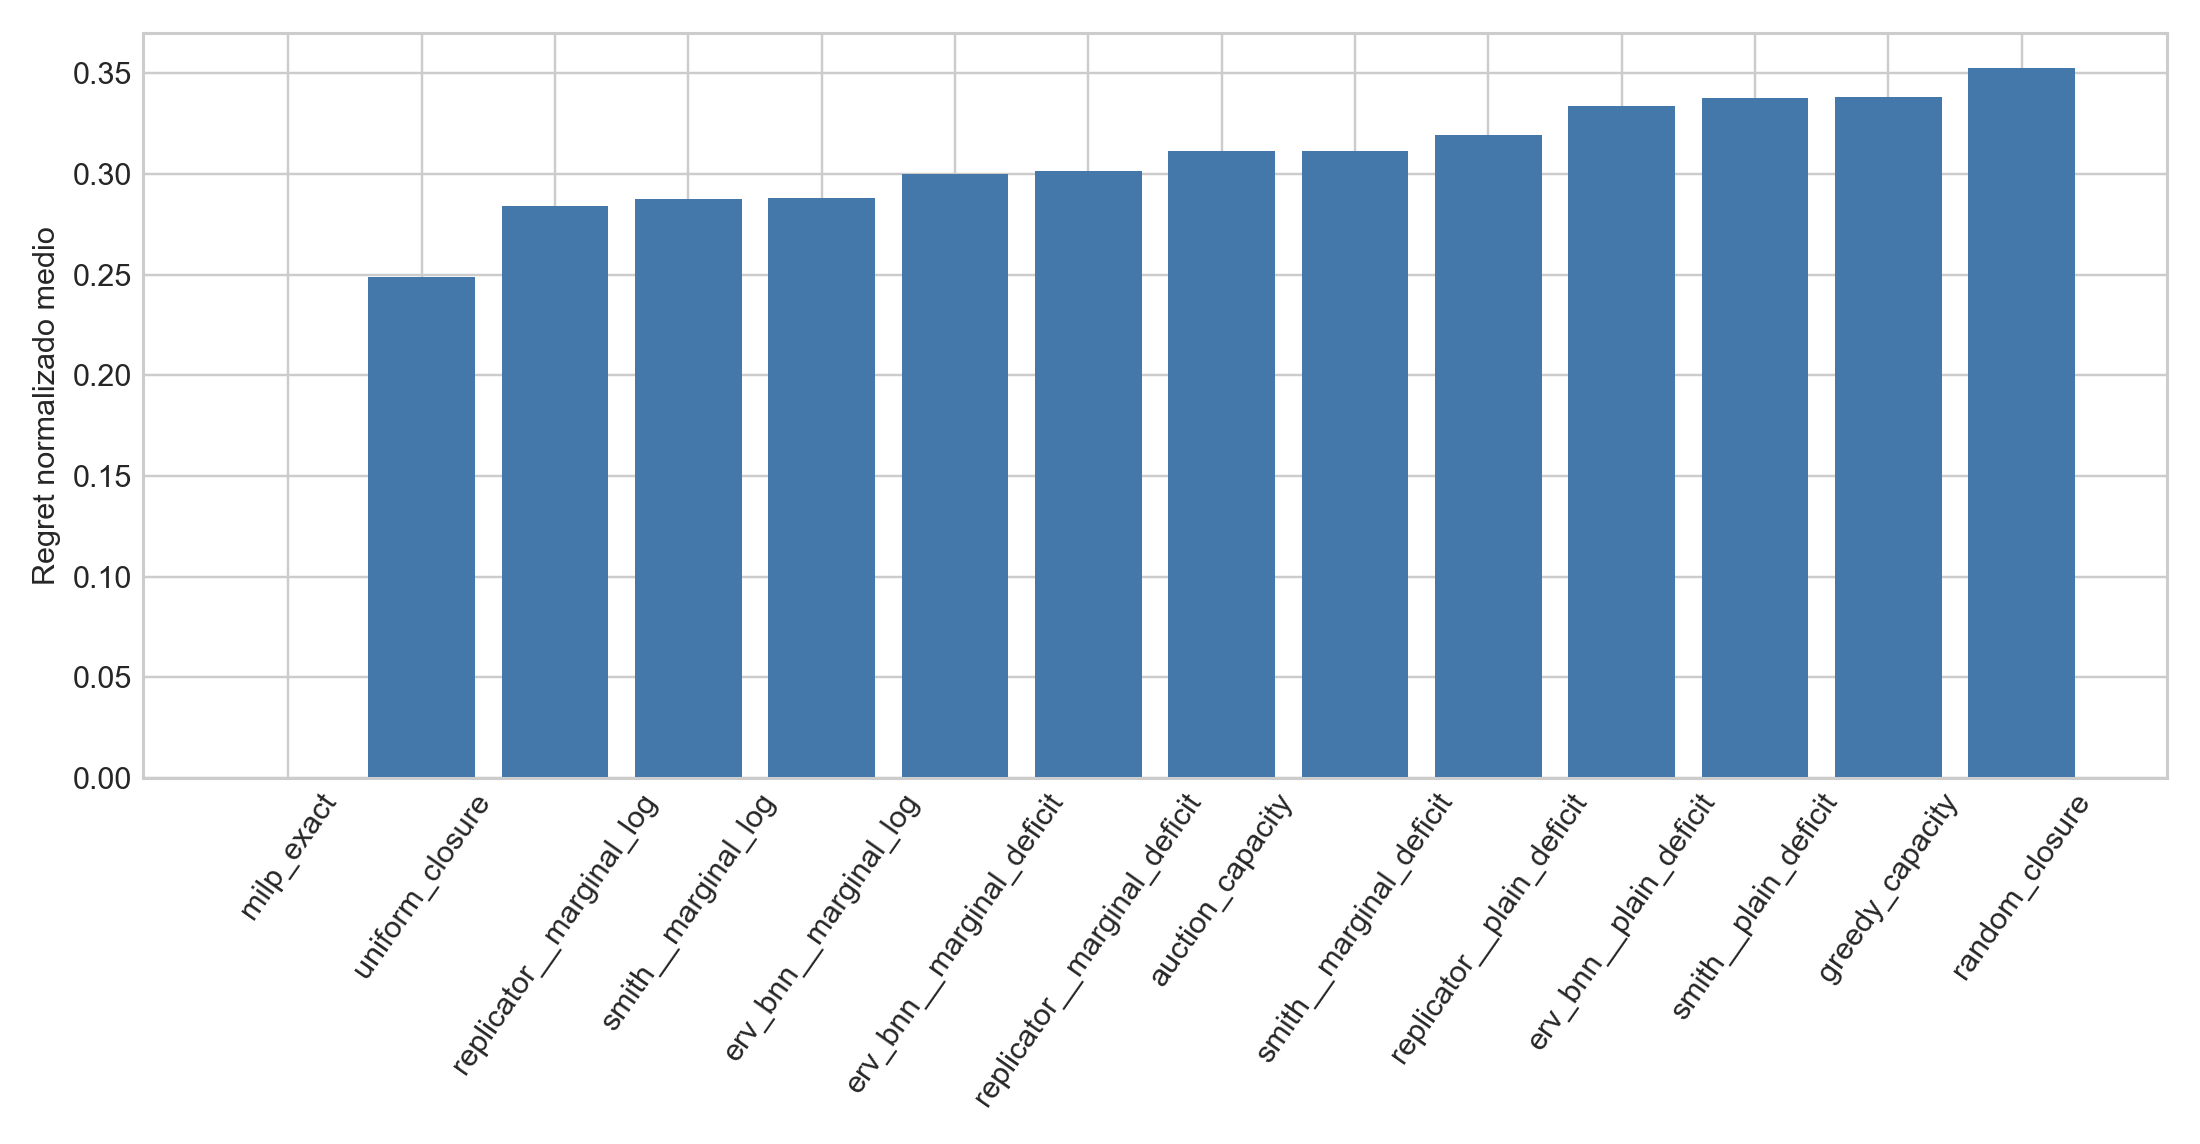
\includegraphics[width=\linewidth]{figures/fig-sp2-heterogeneous-regret.png}
\end{minipage}\hfill
\begin{minipage}[t]{0.49\textwidth}
\centering
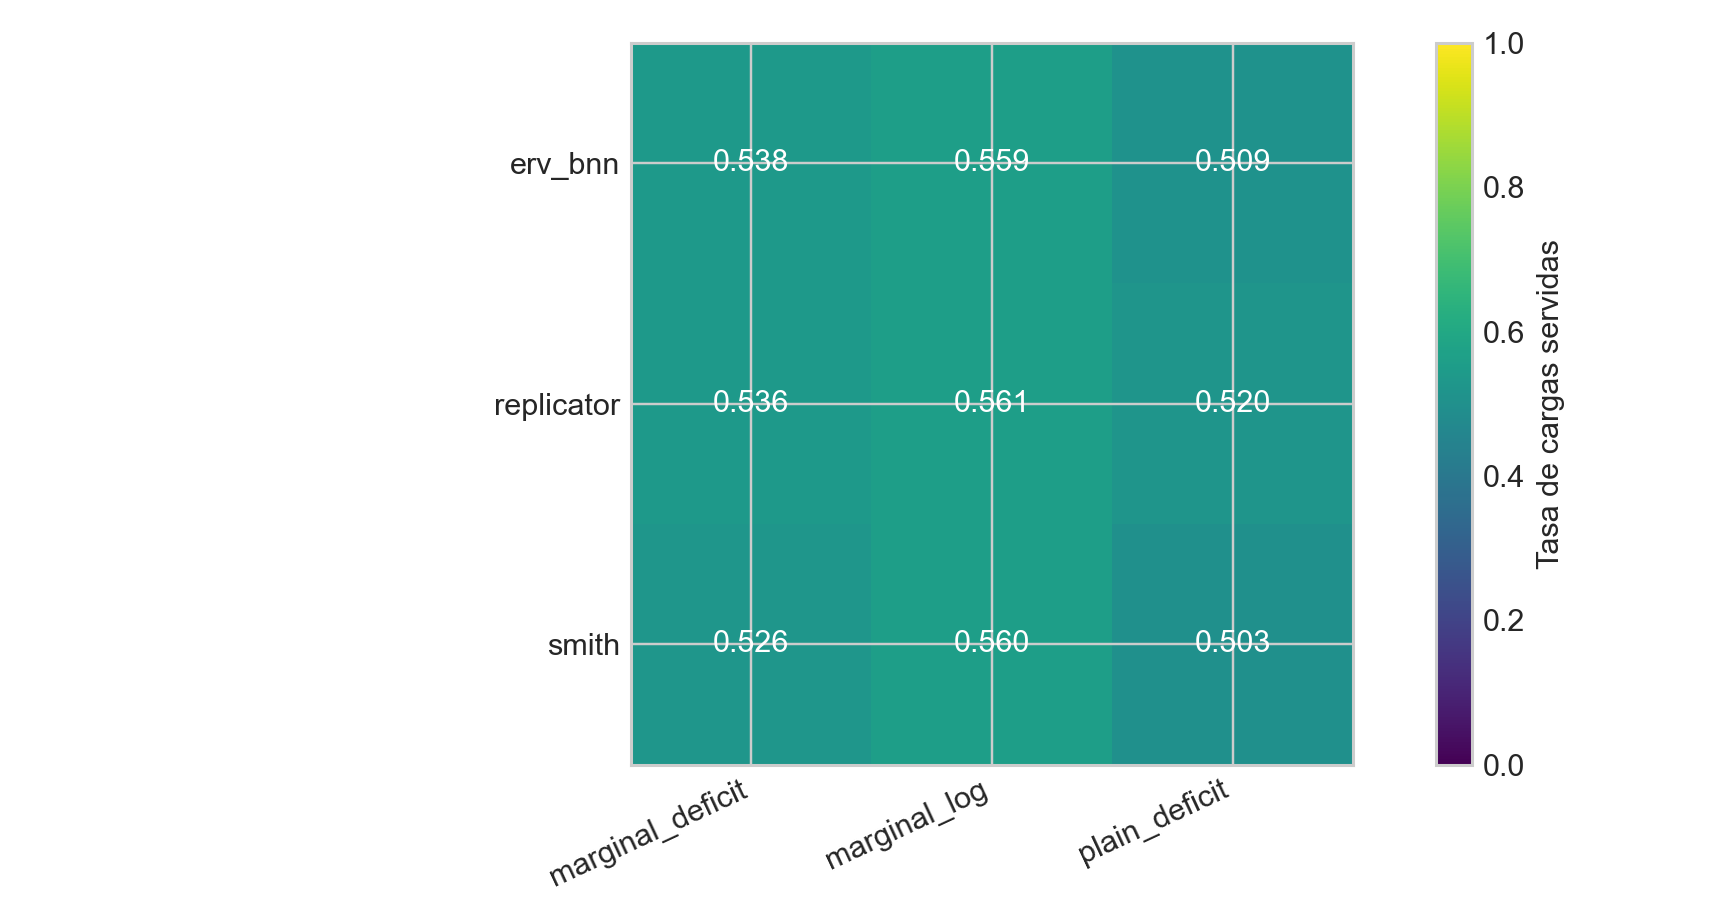
\includegraphics[width=\linewidth]{figures/fig-sp2-fitness-protocol.png}
\end{minipage}
\caption[Resultados factoriales de SP2]{Regret por método e interacción descriptiva entre fitness y protocolo.}
\viuownsource
\label{fig:sp2-heterogeneous-main}
\end{figure}

\subsubsection{Resultados y lectura crítica}

La auditoría terminó en PASS: 4320 ejecuciones poblacionales, 1440 ejecuciones con
potencial exacto e información completa, cero descensos, error máximo del símplex
$4{,}44\times10^{-16}$, residuos finitos, separación RAW/CLOSED, dominancia del
oráculo y emparejamiento completo.

\begin{table}[H]
\centering
\scriptsize
\begin{tabularx}{\textwidth}{@{}p{0.28\textwidth}rrrrr@{}}
\toprule
Método & Servidas & Cobertura & Regret & Conv. & Tiempo (s) \\
\midrule
MILP exacto & 0,8118 & 0,8856 & 0,0000 & 1,000 & 0,0830 \\
Uniforme+closure & 0,5994 & 0,9092 & 0,2489 & 1,000 & 0,0007 \\
Replicator+log & 0,5607 & 0,8819 & 0,2840 & 0,563 & 0,0578 \\
Smith+log & 0,5596 & 0,8805 & 0,2877 & 0,956 & 0,0485 \\
ERV--BNN+log & 0,5589 & 0,8831 & 0,2880 & 1,000 & 0,0440 \\
ERV--BNN+marginal & 0,5383 & 0,8880 & 0,3002 & 0,992 & 0,0409 \\
Subasta proxy & 0,5207 & 0,8875 & 0,3115 & 1,000 & 0,0005 \\
Smith+marginal & 0,5261 & 0,8814 & 0,3115 & 0,950 & 0,0495 \\
Greedy & 0,5342 & 0,7773 & 0,3384 & 1,000 & 0,0009 \\
Aleatorio+closure & 0,5314 & 0,8651 & 0,3524 & 1,000 & 0,0008 \\
\bottomrule
\end{tabularx}
\caption{Resultados finales de SP2 v1.2. El tiempo del MILP incluye construcción y solver.}
\label{tab:sp2-heterogeneous-summary}
\end{table}

Los fitness marginales reducen el regret frente a plain en los tres protocolos. Para
marginal deficit, los efectos son $-0{,}0264$ en Smith, $-0{,}0178$ en replicator y
$-0{,}0338$ en ERV--BNN; los tres sobreviven Holm. Marginal log mejora a plain en
Smith ($-0{,}0502$) y ERV--BNN ($-0{,}0460$). En replicator, el efecto medio es
$-0{,}0356$, pero no supera Holm ($p_{\rm Holm}=0{,}1567$). Esto respalda la necesidad
del factor $e_{ik}$, aunque la función log no domina uniformemente en significación.

No se identifica un protocolo ganador bajo marginal log. ERV--BNN difiere de Smith en
$0{,}0002$ de regret y de replicator en $0{,}0040$; ambos intervalos incluyen cero.
ERV--BNN+log mejora a greedy en $-0{,}0504$ (IC95\%
$[-0{,}0733,-0{,}0289]$), pero su comparación con la subasta no es confirmatoria
($p_{\rm Holm}=0{,}8241$). El MILP conserva una ventaja de $0{,}2880$.

El resultado más importante es negativo. Uniforme+closure logra menor regret que
cualquier juego. El contraste post hoc ERV--BNN+log menos uniforme es $0{,}0391$
(IC95\% $[0{,}0197,0{,}0586]$). Además, uniforme pasa de cero cargas servidas en RAW
a $0{,}5994$ después del cierre. Por tanto, el cierre de capacidad contiene suficiente
información para dominar la preferencia poblacional en esta campaña. No puede afirmarse
que el juego completo supere al mismo decodificador sin señal.

\begin{figure}[H]
\centering
\begin{minipage}[t]{0.49\textwidth}
\centering
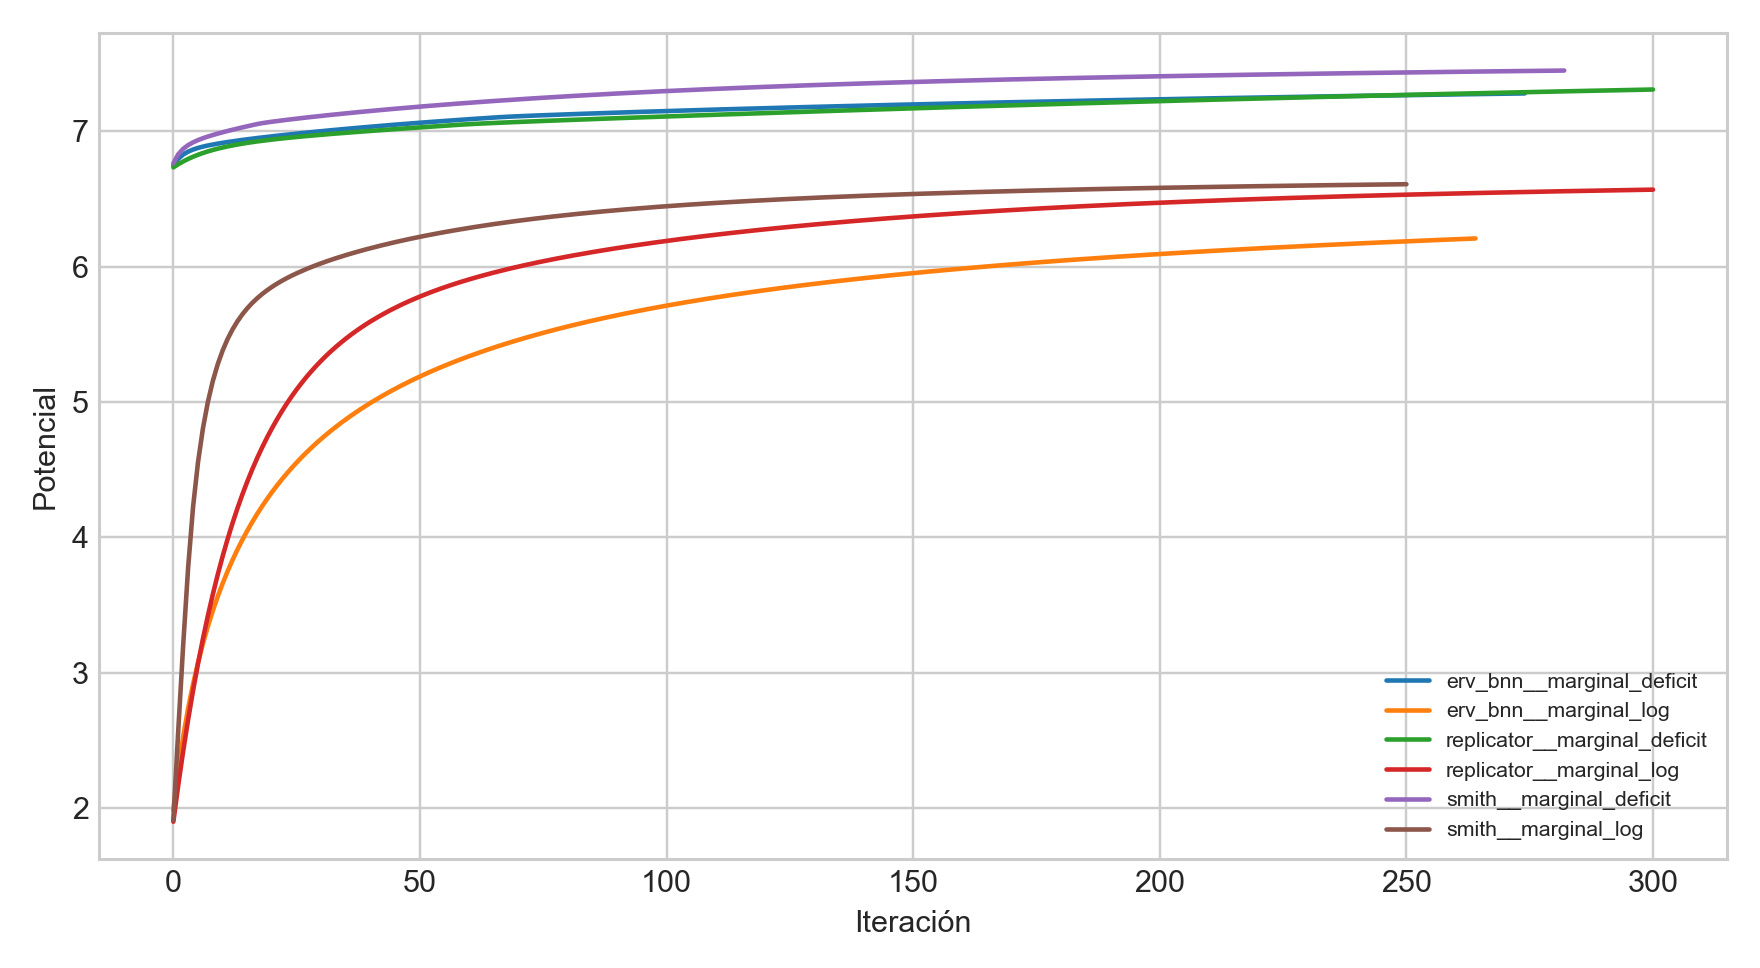
\includegraphics[width=\linewidth]{figures/fig-sp2-potential.png}
\end{minipage}\hfill
\begin{minipage}[t]{0.49\textwidth}
\centering
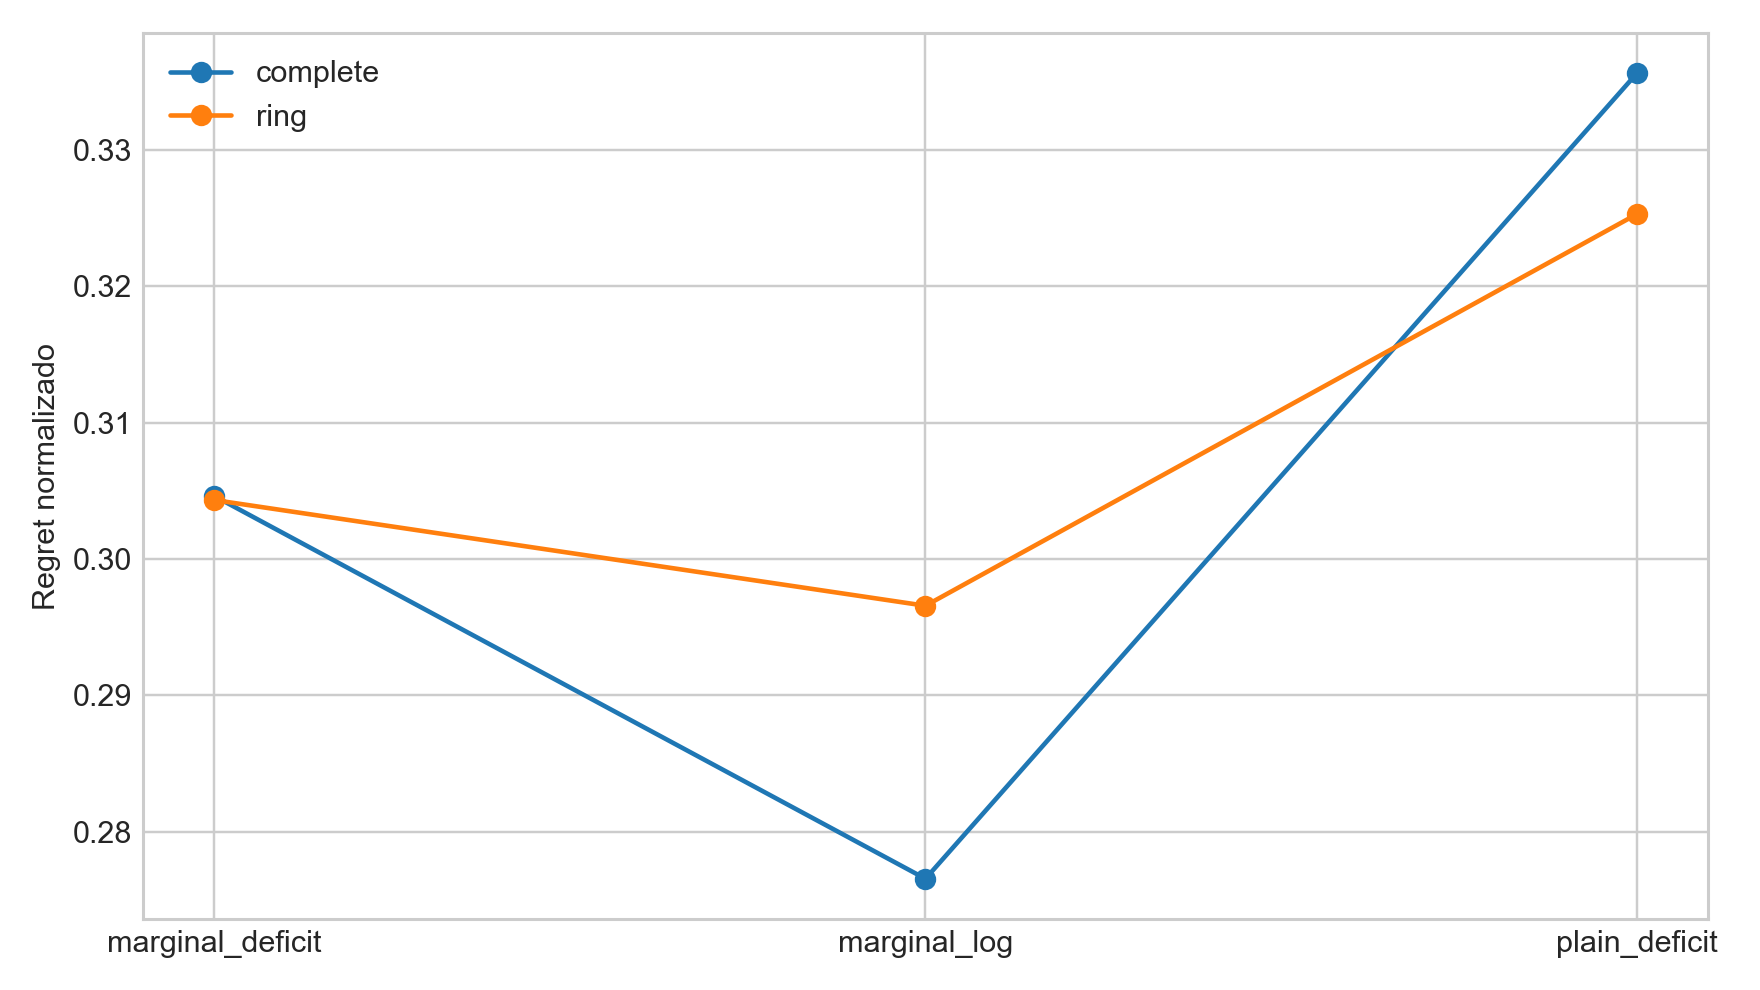
\includegraphics[width=\linewidth]{figures/fig-sp2-graph.png}
\end{minipage}
\caption[Potencial y efecto del grafo en SP2]{Potenciales alineados y sensibilidad a cuatro rondas de consenso en anillo.}
\viuownsource
\label{fig:sp2-heterogeneous-theory}
\end{figure}

El anillo degrada ERV--BNN+log de $0{,}2742$ a $0{,}3017$ de regret y Smith+log de
$0{,}2757$ a $0{,}2998$; replicator cambia de $0{,}2797$ a $0{,}2882$. La demanda
explica una degradación mayor: ERV--BNN+log pasa de $0{,}1403$ con ratio $0{,}70$ a
$0{,}4475$ con ratio $1{,}25$. Estos resultados no demuestran convergencia con grafos
variables ni robustez fuera de las escalas $N\leq16$.

\paragraph{Aporte y límite de SP2.}
La aportación teórica de este nivel es una familia de juegos donde la capacidad
robot--carga aparece en el gradiente marginal, junto con condiciones de potencial,
Nash y complejidad explícitas. La aportación experimental es separar función de fitness,
protocolo de revisión y cierre sobre los mismos mundos. La campaña confirma que el
fitness importa más que elegir Smith, replicator o ERV--BNN. También refuta que esa
mejora baste para superar un cierre heterogéneo fuerte. El siguiente avance debe diseñar
un cierre distribuido o una dinámica cuya variable entera y capacidad residual queden
dentro del juego, no después de él. Finalmente, $e_{ik}$ sigue siendo escalar: no prueba
que una coalición pueda producir fuerza y torque. Esa condición corresponde a SP3.
